\chapter{Supported Hardware Buses} \label{ch:hw_buses}

In this chapter we present the hardware buses to be supported by GEX. The description of each bus is accompanied by several examples of devices that can be interfaced with it. The reader is advised to consult the official specifications and the datasheets of individual sensors and other devices for additional details.

\section{UART and USART} \label{sec:theory_usart}

The \acrfull{USART} has a long history and is still widely used today. This is the frame format used in RS-232, which was once a common way of connecting modems, printers, mice and other devices to personal computers. RS-232 can be considered the ancestor of \gls{USB} in its popularity. \gls{UART} framing is also used in the industrial bus RS-485 and the automotive interconnect bus \gls{LIN}.

\begin{figure}[h]
	\centering
	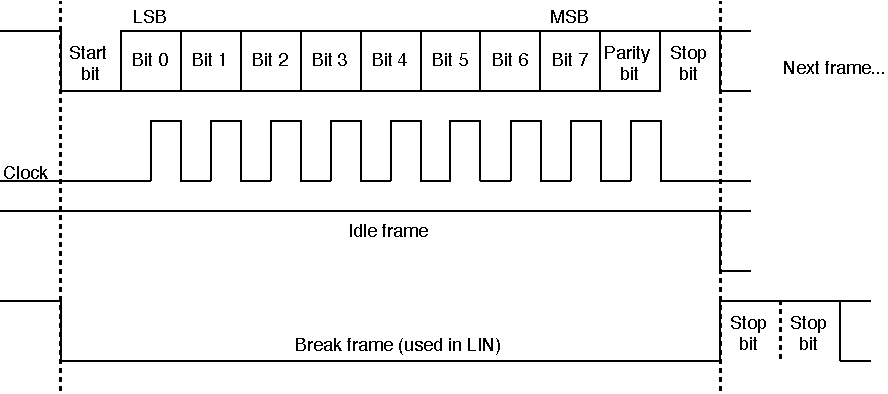
\includegraphics[scale=.9] {img/uart-frame-redraw.pdf}
	\caption[UART frame format]{\label{fig:uart_frame}\gls{USART} frame format in the 8-bit configuration with parity}
\end{figure}

\gls{UART} and \gls{USART} are two variants of the same interface. \gls{USART} includes a separate clock signal, while the \gls{UART} timing relies on a well-known clock speed and the bit clock is synchronized by start bits. \gls{USART} was historically used in modems to achieve higher bandwidth, but is now mostly obsolete.

\gls{USART}, as implemented by microcontrollers such as the STM32 family, is a two-wire full duplex interface that uses 3.3\,V or 5\,V logic levels. The data lines are in the high logical level when idle. A \gls{USART} frame, shown in \cref{fig:uart_frame}, starts by a start-bit (low level for the period of one bit) followed by \textit{n} data bits (typically eight), an optional parity bit, and a period of high level called a stop bit (or stop bits), dividing consecutive frames.

RS-232 uses the \gls{UART} framing, but its levels are different: logical 1 is represented by negative voltages $-3$ to $-25$\,V and logical 0 uses the same range, but positive. To convert between RS-232 levels and \gls{TTL} (5\,V)  or 3.3\,V levels, a level-shifting circuit such as the MAX232 can be used. In RS-232, the two data lines (Rx and Tx) are accompanied by \gls{RTS}, \gls{CTS}, and \gls{DTR}, which facilitate handshaking and hardware flow control. In practice, those additional signals are often unused or their function differs from their historical meaning; for instance, Arduino boards (using a USB-serial converter) use the \gls{DTR} line as a reset signal to automatically enter their bootloader for firmware flashing~\cite{arduinodtr}.

\subsection{Examples of Devices Using UART}

\begin{itemize}
	\item \textbf{MH-Z19B} -- \gls{NDIR} CO$_2$ concentration sensor
	\item \textbf{NEO-M8} -- uBlox \gls{GPS} module
	\item \textbf{ESP8266} with AT firmware -- a WiFi module
	\item \textbf{MFRC522} -- \gls{NFC} MIFARE reader/writer \gls{IC} (also supports other interfaces)
\end{itemize}

\section{SPI} \label{sec:theory_spi}

\acrfull{SPI} is a point-to-point or multi-drop master-slave interface based on shift registers. The \gls{SPI} connection with multiple slave devices is depicted in \cref{fig:spi_multislave}. It uses at least 4 wires: \gls{SCK}, \gls{MOSI}, \gls{MISO} and \gls{SS}. \gls{SS} is often marked \gls{CSB} or \gls{NSS} to indicate that its active state is 0. Slave devices are addressed using their \gls{SS} input while the data connections are shared. A slave that is not addressed releases the \gls{MISO} line to a high impedance state so it does not interfere in ongoing communication.

\begin{figure}[h]
	\centering
	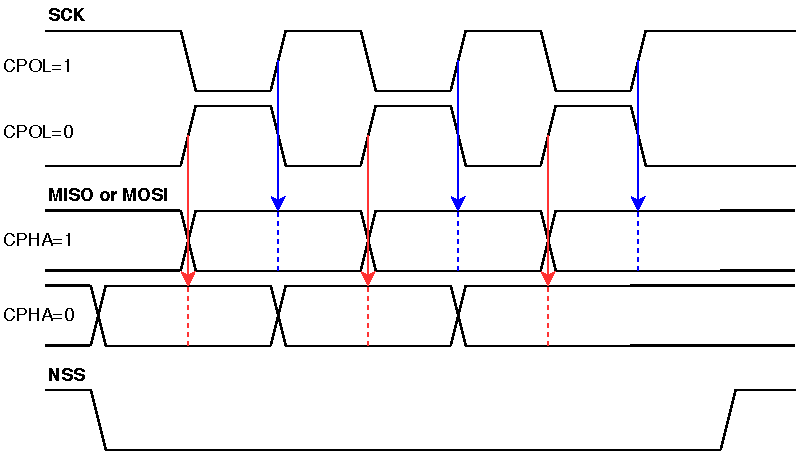
\includegraphics[scale=.9] {img/spi-timing.pdf}
	\caption[SPI timing diagram]{\label{fig:spi_timing}SPI timing diagram explaining the CPOL and CPHA settings (shown on 3 data bits; a real message will use at least 8 bits)}
\end{figure}

\begin{figure}[h]
\centering
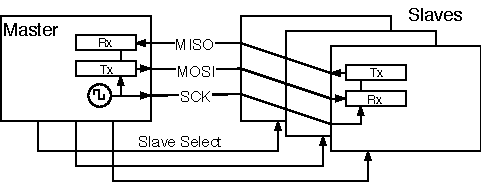
\includegraphics[scale=1.1] {img/spi-multislave-redraw.pdf}
\caption[SPI master with multiple slaves]{\label{fig:spi_multislave}A SPI bus with 1 master and 3 slaves, each enabled by its own Slave Select signal}
\end{figure}

Transmission and reception on the \gls{SPI} bus happen simultaneously. A bus master asserts the \gls{SS} pin of a slave it wishes to address and then sends data on the \gls{MOSI} line while receiving a response on \gls{MISO}. The slave normally responds with 0x00 or a status register as the first byte of the response, before it can process the received command. A timing diagram is shown in \cref{fig:spi_timing}, including two configurable parameters: \gls{CPOL} and \gls{CPHA}.

\gls{SPI} devices often provide a number of control, configuration and status registers that can be read and written by the bus master. The first byte of a command usually contains one bit that determines if it is a read or write access, and an address field selecting the target register. The slave then either stores the following \gls{MOSI} byte(s) into the register, or sends its content back on \gls{MISO} (or both simultaneously).

\pagebreak[1] % TODO
\subsection{Examples of Devices Using SPI}

\begin{itemize}
	\item \textbf{SX1276} -- LoRa transceiver
	\item \textbf{nRF24L01+} -- 2.4\,GHz ISM band radio module
	\item \textbf{L3GD20} -- 3-axis gyroscope
	\item \textbf{BMP280} -- pressure sensor
	\item \textbf{BME680} -- air quality sensor
	\item \textbf{ENC28J60} -- Ethernet controller
	\item \textbf{L6470} -- intelligent stepper motor driver
	\item \textbf{AD9833} -- waveform generator (\gls{MOSI} only)
	\item \textbf{ADE7912} -- triple $\Sigma$-$\Delta$ \gls{ADC} for power metering applications
	\item \textbf{SD cards}~\cite{sd-spec}
	\item SPI-interfaced EEPROM and Flash memories
\end{itemize}

\section{\texorpdfstring{\IIC}{I2C}} \label{sec:theory_i2c}

\acrfull{I2C} is a two-wire, open-drain bus that supports multi-master operation.
It uses two connections (plus \gls{GND}): \gls{SDA} and \gls{SCL}, both open-drain with a pull-up resistor.

The protocol was developed by Philips Semiconductor (now NXP Semiconductors), and its implementors were, until 2006, required to pay licensing fees, leading to the development of compatible implementations with different names, such as Atmel's \gls{TWI} or Dallas Semiconductor's ``Serial 2-wire Interface'' (e.g., used in the DS1307 \gls{RTC} chip). \gls{I2C} is a basis of the \gls{SMBus} and \gls{PMBus}, which add additional constraints and rules for a more robust operation.

The frame format is shown and explained in \cref{fig:i2c_frame}; more details may be found in the specification~\cite{i2c-spec} or application notes and datasheets offered by chip vendors, such as the white paper from Texas Instruments~\cite{understanding-i2c}. A frame starts with a start condition and stops with a stop condition, defined by an \gls{SDA} edge while the \gls{SCL} is high. The address and data bytes are acknowledged by the slave by sending a 0 on the open-drain \gls{SDA} line in the following clock cycle. A slave can terminate the transaction by sending 1 in place of the acknowledge bit. Slow slave devices may stop the master from sending more data by holding the SCL line low at the end of a byte, a feature called \textit{Clock Stretching}. As the bus is open-drain, the line cannot go high until all participants release it.

Two addressing modes are defined: 7-bit and 10-bit. Due to the small address space, exacerbated by many devices implementing only the 7-bit addressing, collisions between different chips on a shared bus are common; many devices thus offer several pins to let the board designer choose a few bits of the address by connecting them to different logic levels.

The bus supports multi-master operation, which leads to the problem of collisions. Multi-master capable devices must implement a bus arbitration scheme as specified by the \gls{I2C} standard~\cite{i2c-spec}. This feature is, however, rarely used in practice; the most common topology for \gls{I2C} is multi-drop single-master, similar to \gls{SPI}, with the advantage of using only two microcontroller pins.

\begin{figure}[h]
	\centering
	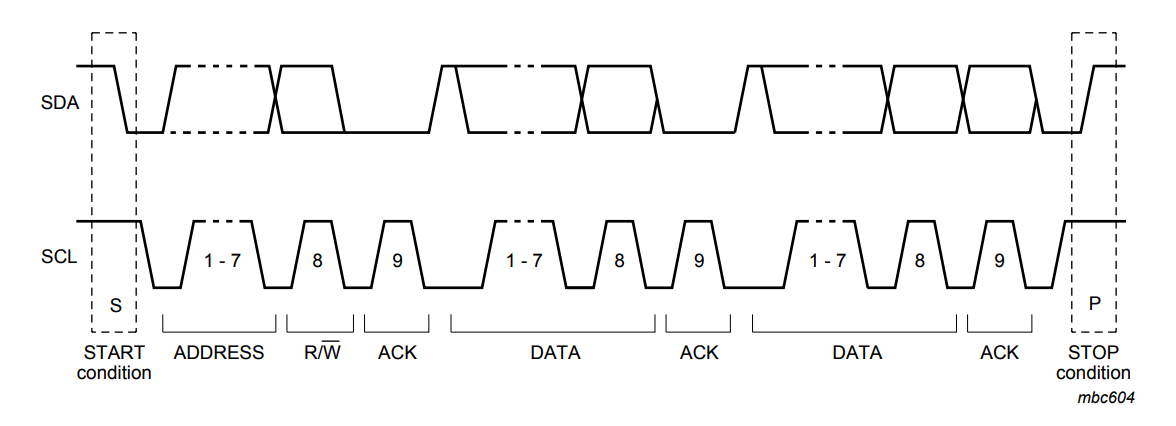
\includegraphics[width=.9\textwidth] {img/i2c-frame.png}
	\caption[\IIC message diagram]{\label{fig:i2c_frame}An \gls{I2C} message diagram (\textit{taken from the \gls{I2C} specification~\cite{i2c-spec}})}
\end{figure}

\subsection{Examples of Devices Using \texorpdfstring{\IIC}{I2C}}

\begin{itemize}
	\item \textbf{APDS-9960} -- ambient light, proximity and gesture sensor
	\item \textbf{L3GD20}, \textbf{BMP280}, \textbf{BME680} -- listed as \gls{SPI} devices, those also support \gls{I2C}
	\item \textbf{DS1307} -- \gls{RTC}; \gls{I2C} is not mentioned in the entire datasheet, presumably to avoid paying license fees, but it is fully compatible
	\item \textbf{IS31FL3730} -- a \gls{LED} matrix driver
	\item The \gls{SCCB} used to configure camera modules is derived from \gls{I2C}
\end{itemize}

\section{1-Wire} \label{sec:theory_1wire}

The 1-Wire bus, developed by Dallas Semiconductor (acquired by Maxim Integrated), uses a single, bi-directional data line (\cref{fig:1w_topology}), which can also power the slave devices in a \textit{parasitic mode}, reducing the number of required wires to just two (compare with 3 in \gls{I2C} and 5 in \gls{SPI}, all including \gls{GND}). The parasitic operation is possible thanks to the data line resting at a high logic level most of the time, charging an internal capacitor.

1-Wire uses an open-drain connection for the data line, similar to \gls{I2C}, though the protocol demands it to be connected directly to V$_dd$ in some places when the parasitic mode is used; this is accomplished using an external transistor, or by reconfiguring the GPIO pin as output and setting it to 1, provided the microcontroller is able to supply a sufficient current.

The communication consists of short pulses sent by the master and (for bit reading) the line continuing to be held low by the slave for a defined amount of time. The pulse timing determines whether it is a read or write operation and which value is encoded. It can be implemented either in software as delay loops, or by abusing a \gls{UART} peripheral, as explained in~\cite{ow-uart}. Detailed timing diagrams can be found in the DS18x20~\cite{ow-datasheet}. 1-Wire transactions include a checksum byte to ensure an error-free communication.

\begin{figure}[h]
	\centering
	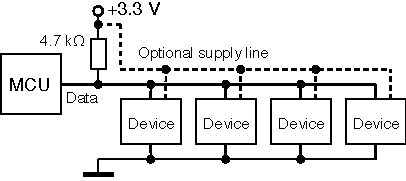
\includegraphics[scale=1] {img/1w-connection.pdf}
	\caption{\label{fig:1w_topology}1-Wire connection topology with four slave devices}
\end{figure}

Devices are addressed by their unique 64-bit ID numbers called ROM codes or ROMs; they can be found by the bus master, with a cooperation from slaves, using a ROM Search algorithm. The search algorithm is explained in~\cite{ow-appnote}, including a possible implementation example. If only one device is connected, a wild card command Skip ROM can be used to address the device without a known ROM code.

\subsection{Examples of Devices Using 1-Wire}

\begin{itemize}
	\item \textbf{DS1820}, \textbf{DS18S20}, \textbf{DS18B20} -- digital thermometers
	\item \textbf{iButton} -- contact-read access tokens, temperature loggers, etc.
\end{itemize}

Since 1-Wire is a proprietary protocol, there is a much smaller choice of available devices and they also tend to be more expensive. The DS18x20 thermometers are, however, popular enough to warrant the bus's inclusion in GEX.

\iffalse
\begin{figure}[h]
	\centering
	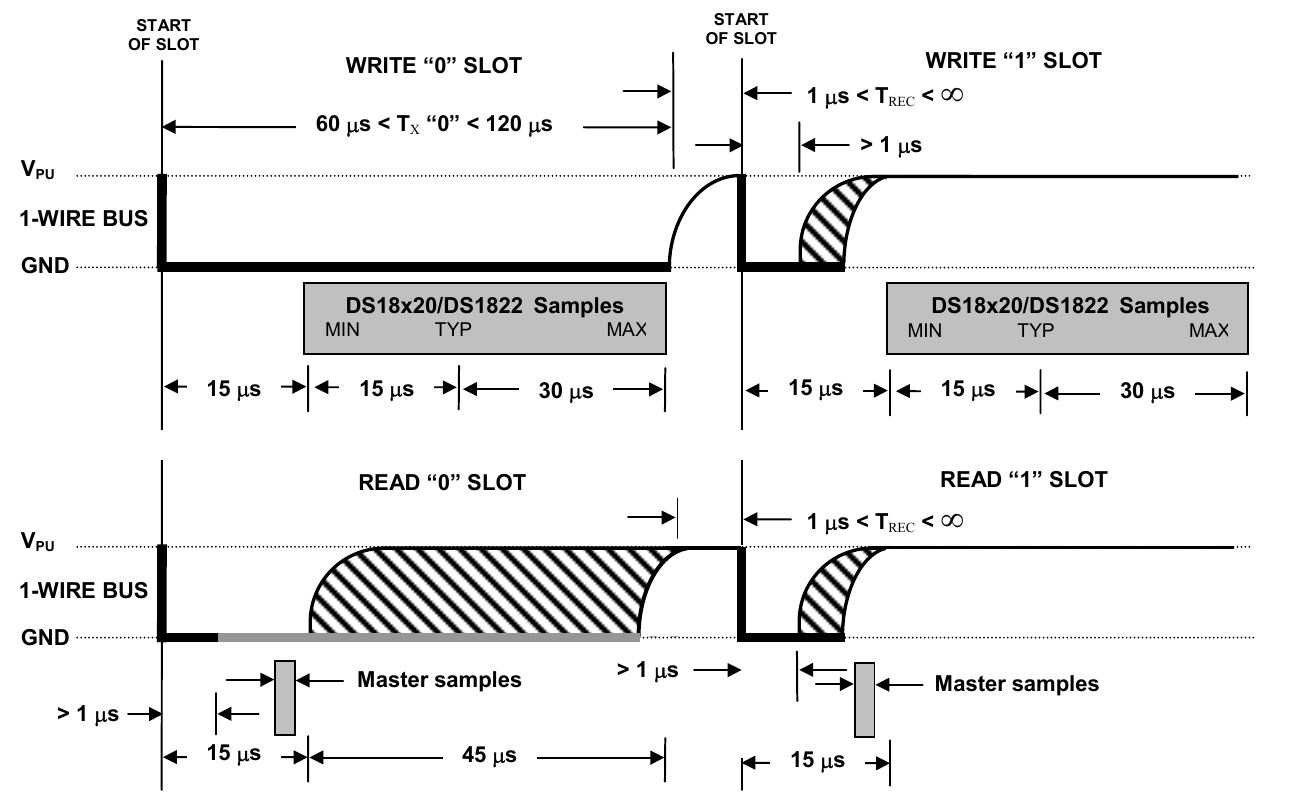
\includegraphics[width=.85\textwidth] {img/1w-rw.png}
	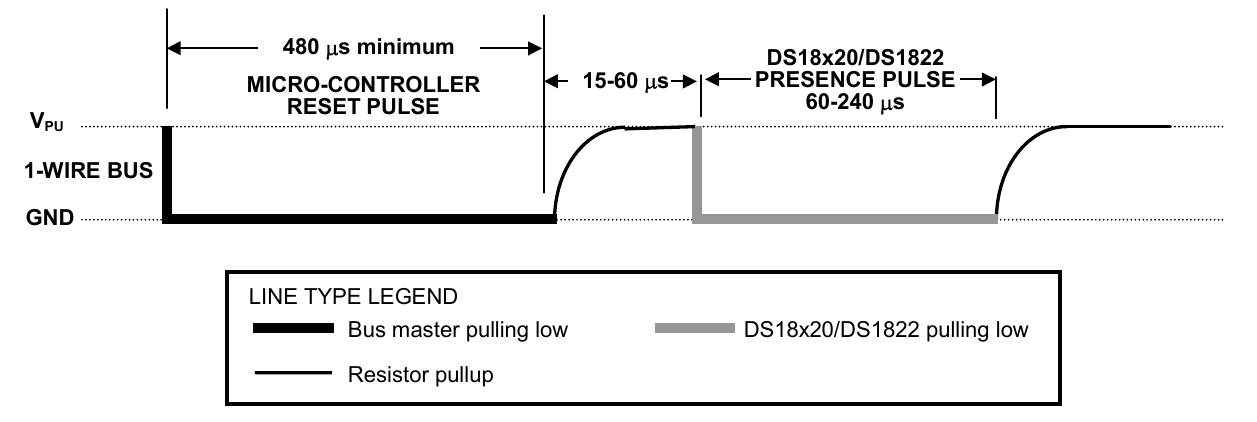
\includegraphics[width=.85\textwidth] {img/1w-reset.png}
	\caption{\label{fig:1w_pulses}The 1-Wire data line pulse timing (by \textit{Dallas Semiconductor})}
\end{figure}
\fi


\section{NeoPixel} \label{sec:theory_neo}

NeoPixel is a marketing name of the \textbf{WS2812} and compatible intelligent \gls{LED} drivers that are commonly used in ``addressable \gls{LED} strips'' (\cref{fig:neopic}).  These chips include the control logic, PWM drivers and the \gls{LED} diodes all in one 5$\times$5\,mm SMD package.

The NeoPixel protocol is unidirectional, using only one data pin. The \gls{LED} drivers are chained together. Ones and zeros are encoded by pulses of a defined length on the data pin; after the color data was loaded into the \gls{LED} string, a longer ``reset'' pulse (low level) is issued by the bus master and the set colors are displayed. The timing constraints are listed in \cref{fig:ws2812_dia}.

The NeoPixel timing is sensitive to pulse length accuracy; a deviation from the specified timing may cause the data to be misinterpreted by the drivers. Some ways to implement the timing use hardware timers or the \gls{I2S} peripheral. An easier method that does not require any additional hardware resources beyond the \gls{GPIO} pin is to implement the timing using delay loops in the firmware; care must be taken to disable interrupts in the sensitive parts of the timing; it may be advantageous to implement it in assembly for a tighter control.

\iffalse
\begin{figure}[h]
	\centering
	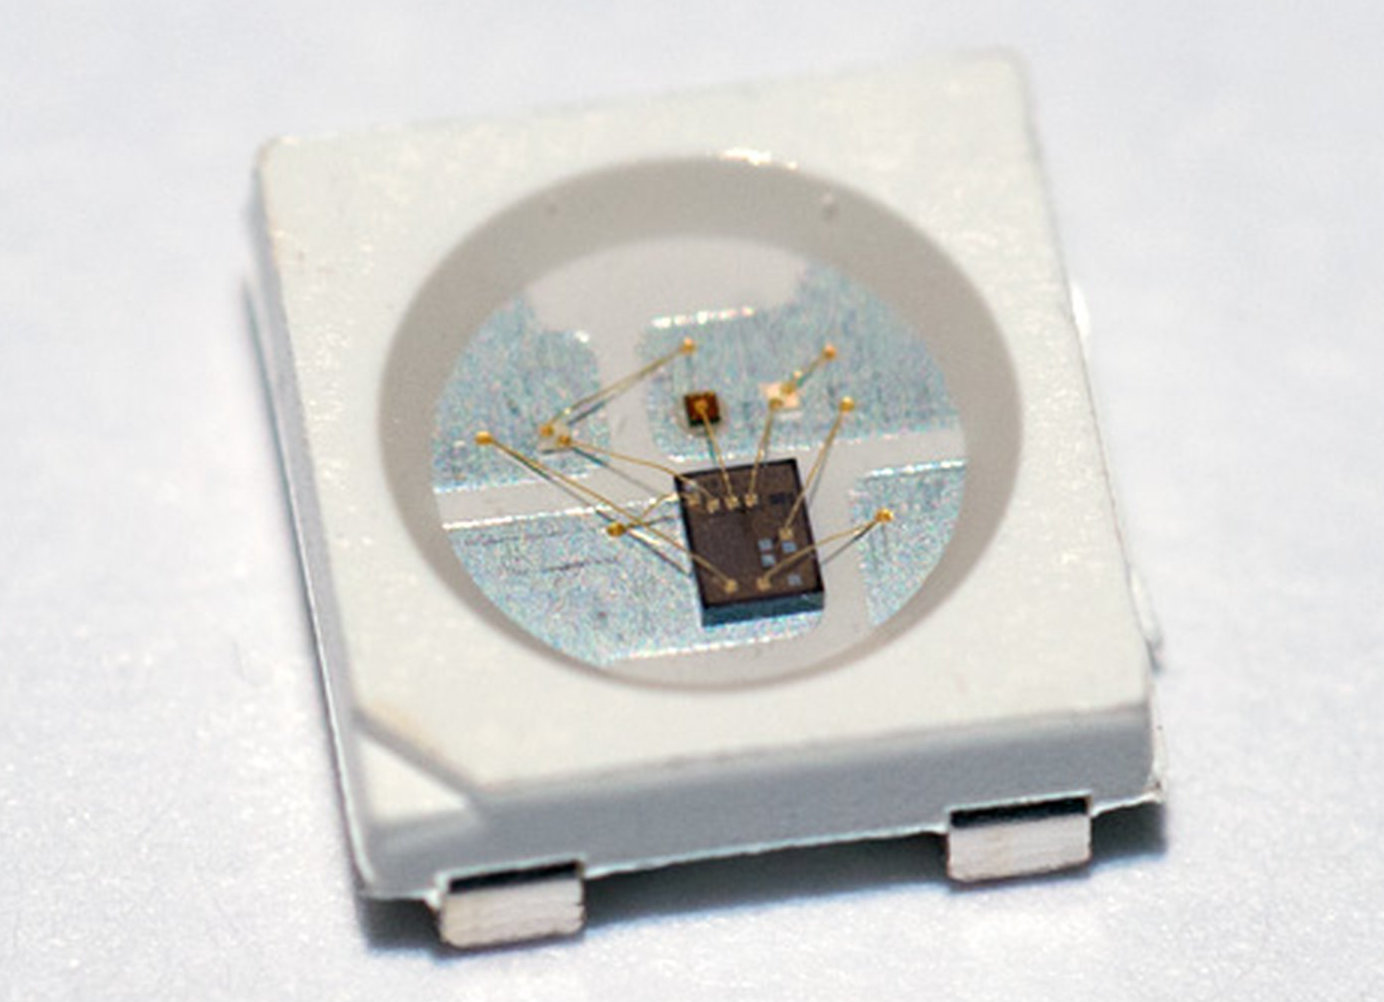
\includegraphics[width=.5\textwidth] {img/ws2812b-detail.jpg}
	\caption{\label{fig:ws2812_detail}A close-up photo of a WS2812B pixel, showing the LED driver IC}
\end{figure}
\fi

\begin{figure}[h]
	\centering
	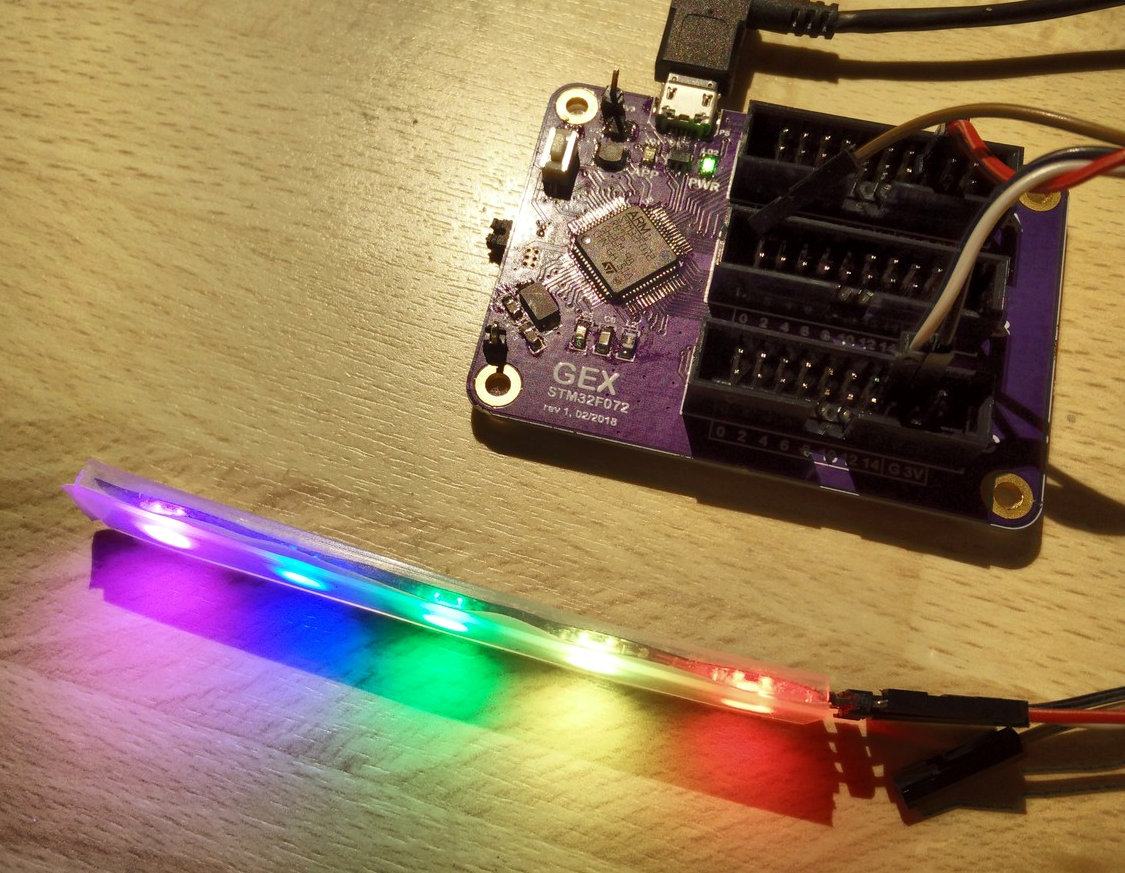
\includegraphics[width=.7\textwidth] {img/npxdriven.jpg}
	\caption{\label{fig:neopic}GEX prototype driving a strip of 5 NeoPixels}
\end{figure}

\begin{table}[h]
	\centering
	\begin{tabular}{cll}
		\toprule
		\textbf{Bit value} & \textbf{Constraint} & \textbf{Duration} \\
		\midrule
		0 & High level & $0.4\,\mu\mathrm{s}\pm150\mathrm{ns}$ \\
		0 & Low level & $0.85\,\mu\mathrm{s}\pm150\mathrm{ns}$ \\
		1 & High level & $0.45\,\mu\mathrm{s}\pm150\mathrm{ns}$ \\
		1 & Low level & $0.8\,\mu\mathrm{s}\pm150\mathrm{ns}$ \\
		-- & Reset pulse (low) & $>50\,\mu\mathrm{s}$ \\
		\bottomrule
	\end{tabular}
%	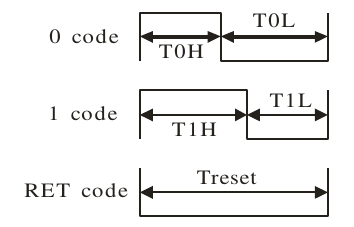
\includegraphics[width=.4\textwidth] {img/neo-diagram.png}
%	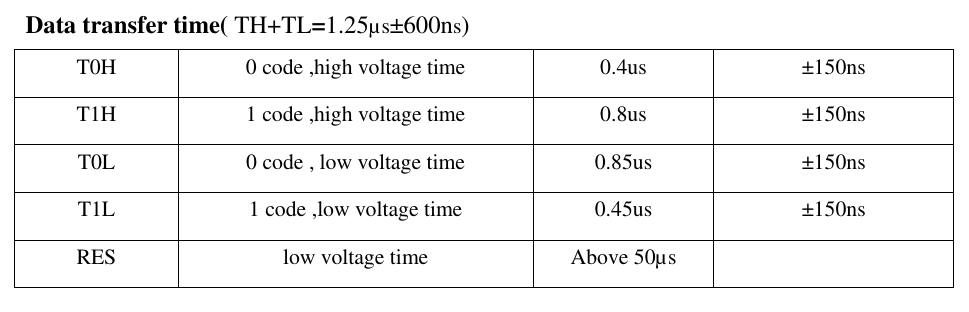
\includegraphics[width=\textwidth] {img/neo-lengths.png}
	\caption{\label{fig:ws2812_dia}NeoPixel pulse timing}
	%TODO reference
\end{table}




